\documentclass[12pt]{article}

\usepackage{graphicx}
\usepackage{amsmath}
\usepackage{amssymb}
\usepackage{natbib}
\usepackage{amsfonts}
\usepackage{multicol}
\usepackage{float}
\usepackage{oldgerm}
\usepackage{bm}
\usepackage{mathtools}
\usepackage{wrapfig}
\usepackage{fancyhdr}
\usepackage[export]{adjustbox}
\usepackage{xcolor}

\pagestyle{empty}

\newcommand{\Avec}{\mathbf A}
\newcommand{\Bvec}{\mathbf B}
\newcommand{\Dvec}{\mathbf D}
\newcommand{\Evec}{\mathbf E}
\newcommand{\Fvec}{\mathbf F}
\newcommand{\Jvec}{\mathbf J}
\newcommand{\Lvec}{\mathbf L}
\newcommand{\Mvec}{\mathbf M}
\newcommand{\Pvec}{\mathbf P}
\newcommand{\Rvec}{\mathbf R}
\newcommand{\Svec}{\mathbf S}
\newcommand{\Tvec}{\mathbf T}
\newcommand{\avec}{\mathbf a}
\newcommand{\bvec}{\mathbf b}
\newcommand{\dvec}{\mathbf d}
\newcommand{\evec}{\mathbf e}
\newcommand{\fvec}{\mathbf f}
\newcommand{\jvec}{\mathbf j}
\newcommand{\kvec}{\mathbf k}
\newcommand{\nvec}{\mathbf n}
\newcommand{\pvec}{\mathbf p}
\newcommand{\rvec}{\mathbf r}
\newcommand{\svec}{\mathbf s}
\newcommand{\vvec}{\mathbf v}
\newcommand{\xvec}{\mathbf x}
\newcommand{\yvec}{\mathbf y}
\newcommand{\zvec}{\mathbf z}
\newcommand{\nablav}{\boldsymbol{\nabla}}
\newcommand{\nablavector}{\vec \nabla}
\newcommand{\alphavec}{\boldsymbol{\alpha}}
\newcommand{\phivec}{\boldsymbol{\phi}}
\newcommand{\thetavec}{\boldsymbol{\theta}}
\newcommand{\omegavec}{\boldsymbol{\omega}}
\newcommand{\tauvec}{\boldsymbol{\tau}}
\newcommand{\ezero}{\varepsilon_{0}}
\newcommand{\mzero}{\mu_{0}}
\newcommand{\mubold}{\boldsymbol{\mu}}
\newcommand{\uniti}{\hat{\boldsymbol{\imath}}}
\newcommand{\unitj}{\hat{\boldsymbol{\jmath}}}
\newcommand{\unitk}{\hat{\boldsymbol{\mathit{k}}}}
\newcommand{\unitn}{\hat{\mathbf n}}
\newcommand{\unitr}{\hat{\mathbf r}}
\newcommand{\unitphi}{\hat{\boldsymbol{\phi}}}
\newcommand{\unittheta}{\hat{\boldsymbol{\theta}}}


\newcommand{\bit}{\begin{itemize}}
\newcommand{\eit}{\end{itemize}}

\setlength{\headsep}{0.5cm}
\setlength{\oddsidemargin}{-0.5cm}
\setlength{\textwidth}{16.5cm}
\setlength{\textheight}{24cm}
\voffset = -2cm


\pagestyle{fancy}
\fancyhf{}
\rfoot{
\includegraphics[width=1.0in]{cnm.png}}
\lfoot{Homework 3}
\begin{document}

%{\bf \underline{STUDENT NAME}:} 
%\vspace{1cm}

\begin{center}
%\date{10/02/18-10/09/18}
\hfil
{\large\bf {ENGR 2910-101: Circuit Analysis}}
\hfill Instructor: Leo Silbert \\
Homework 2: 09/07/21 \hfill Due: 09/14/21\\
\hrulefill\\
\end{center}

%{\em Show all your working to ensure you obtain full points. Partial
%  credit will be given for correct algebraic steps if you fail to
%  obtain the correct final answer.}\\

%\newpage


\noindent
{\bf Question 1} [10] %P2-1

If the interconnection in the figure below is valid, find the power developed in the current sources. Whether the circuit is valid or not, either way provide an explanation why.
\begin{figure}[h!]
  \centering 
  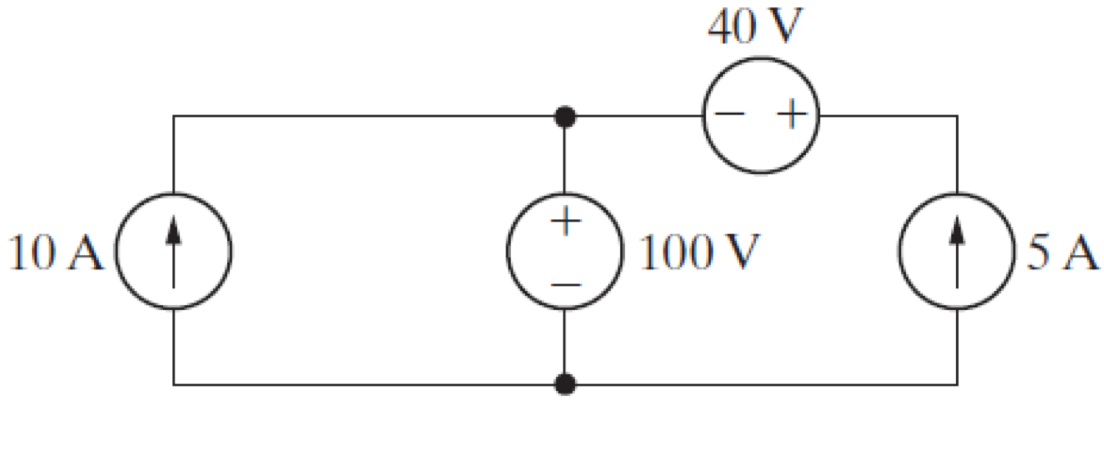
\includegraphics[clip,width=0.5\textwidth]{P2-1.png}
\end{figure}

\vspace{0.1in}
\noindent
{\bf Question 2} [10] %P2-3

If the interconnection in the figure below is valid, find the power developed in the voltage sources. Whether the circuit is valid or not, either provide an explanation why.
\begin{figure}[h!]
  \centering 
  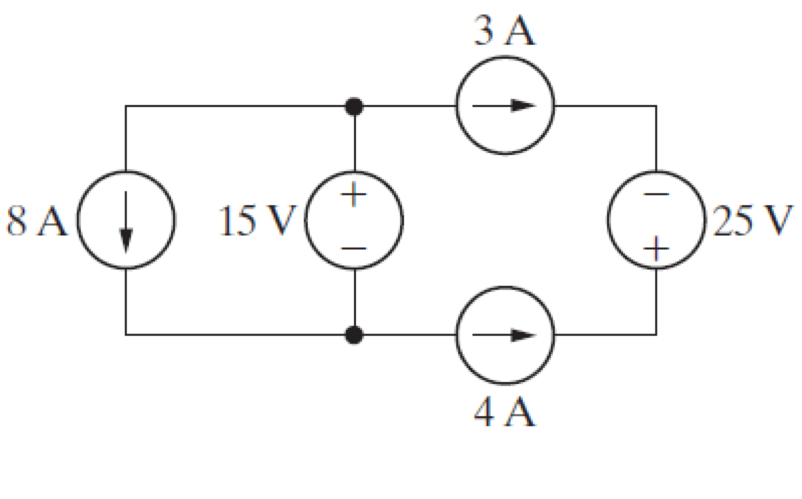
\includegraphics[clip,width=0.5\textwidth]{P2-3.png}
\end{figure}

\vspace{0.1in}
\noindent
{\bf Question 3} [10] %P2-9

Find the total power developed in the circuit if $v_{o} = 5$ V.
\begin{figure}[h!]
     \centering
     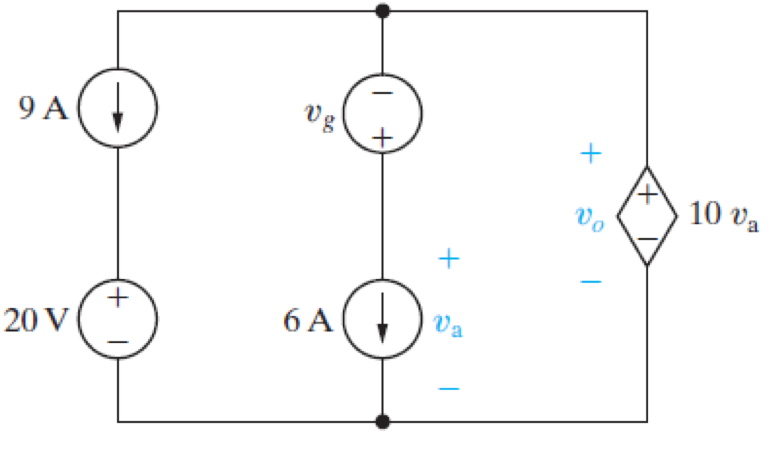
\includegraphics[clip,width=0.6\textwidth]{P2-9.png}
\end{figure}
 

\vspace{0.1in}
\noindent
{\bf Question 4} [10] %P2-13

A pair of automotive headlamps is connected to a 12 V battery as shown below. The symbol $\blacktriangledown$ indicates that the terminal is connected directly to the metal frame of the car. [Hint: take into account internal resistance and resistances of wires and between other connectors.]
\begin{figure}[h!]
  \centering 
  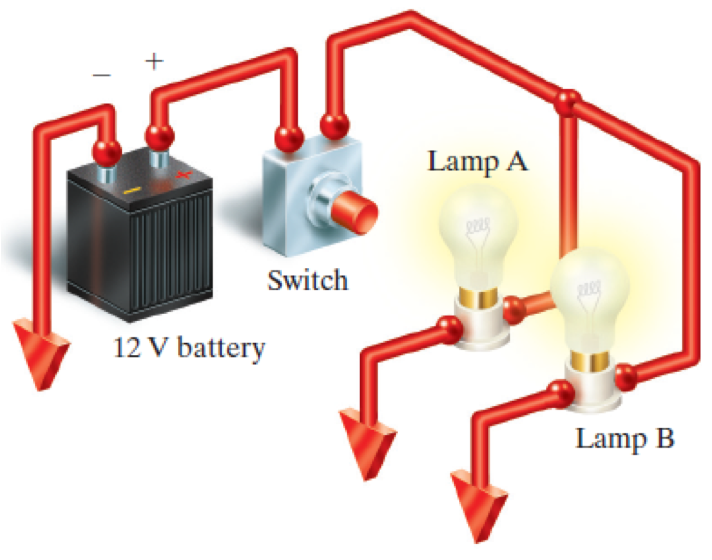
\includegraphics[clip,width=0.3\textwidth]{P2-13.png}
\end{figure}

\bit

\item[(a)]

Construct a circuit model using resistors and an independent voltage source. 

\item[(b)]

Identify and list the correspondence between the ideal circuit element and the ymbol component that it represents in the figure.

\eit


\vspace{0.1in}
\noindent
{\bf Question 5} [10] %P2-14

The terminal voltage and terminal current were measured (b) on the device (a) shown. Construct a circuit model for the device consisting of a single resistor. Provide a graph (either hand-drawn or software generated) showing how you determine the value of the resistor. 
\begin{figure}[h!]
\centering 
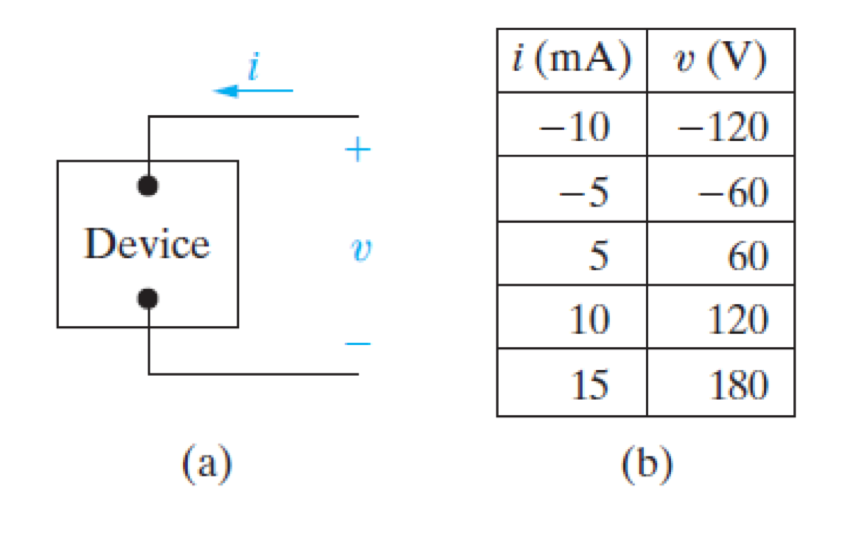
\includegraphics[clip,width=0.49\textwidth]{P2-14.png}
\end{figure}
 

\end{document}
